%++++++++++++++++++++++++++++++++++++++++
% Don't modify this section unless you know what you're doing!
\documentclass[a4paper,12pt]{article}
\usepackage{listings} % code blocks
\usepackage{tabularx} % extra features for tabular environment
\usepackage{amsmath}  % improve math presentation
\usepackage{graphicx} % takes care of graphic including machinery
\usepackage{subcaption} % necessary for subfigures
\usepackage{float}
\usepackage[margin=3.0cm,a4paper]{geometry} % decreases margins
%\usepackage{cite} % takes care of citations
%\usepackage[final]{hyperref} % adds hyper links inside the generated pdf file
%++++++++++++++++++++++++++++++++++++++++

\setlength{\parindent}{0pt}
\usepackage{hyperref}

\begin{document}

\title{Deep Learning Lab \\ Exercise 04 }
\author{Rabea Turon \& Megan Klaiber}
\date{\today}
\maketitle

\section{Introduction}

In this exercise a DQN agent will be implemented and its prformance willl be evaluated on the CartPole and CarRacing environment of OpenAI Gym.


\section{Reinforcement Learning: Deep Q-Networks}\label{rl}


\subsection{CartPole}\label{cartpole}

A simple neural network was used for the CartPole task. It consists of two fully connected layers each with 20 hidden units. The network is optimized with mean squared error and Adam optimizer. CartPole is considered solved when the average reward is greater than or equal to 195.0 over 100 consecutive episodes. So we stopped the training when this point was reached. The size of the batches sampled from the replay buffer was 64 and we used a learning rate of 0.001.\\

\autoref{fig:cartpole_episode_reward} shows the achieved reward during the training episodes. Here CartPole was solved after 150 episodes. During training every 20th episode the agent was evaluated with deterministic actions over 5 episodes. The average reward of these 5 episodes is shown in \autoref{fig:cartpole_evaluation_reward}. The final performance was evaluated over 15 test episodes. Here the average reward was 349 with a standard deviation of 72.


\begin{figure}[H]
	\centering 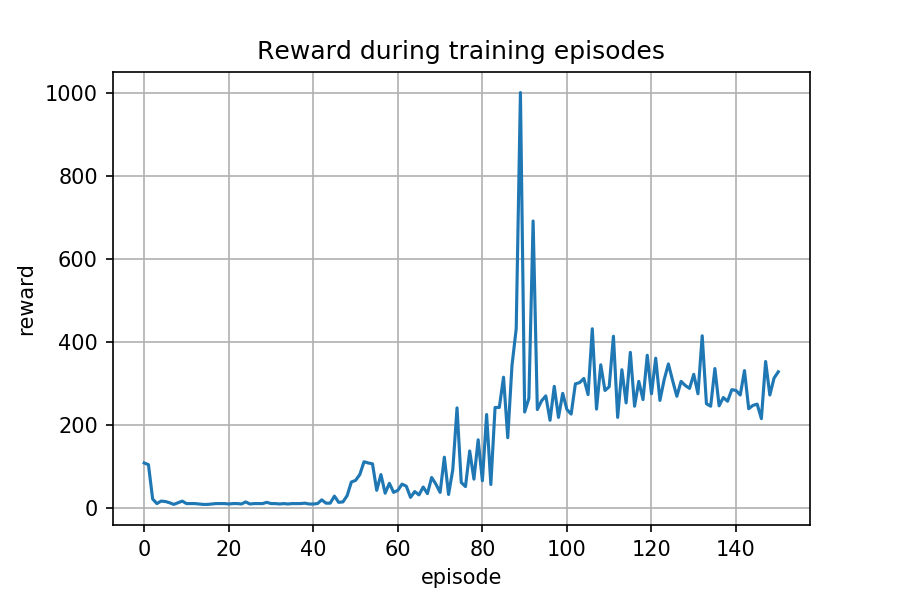
\includegraphics[width=11.70cm, height=7.9cm]{plots/cartpole_episode_reward.png}
	\caption{
		\label{fig:cartpole_episode_reward}
		Achieved reward during training episodes of CartPole.
	}
\end{figure}

\begin{figure}[H]
	\centering 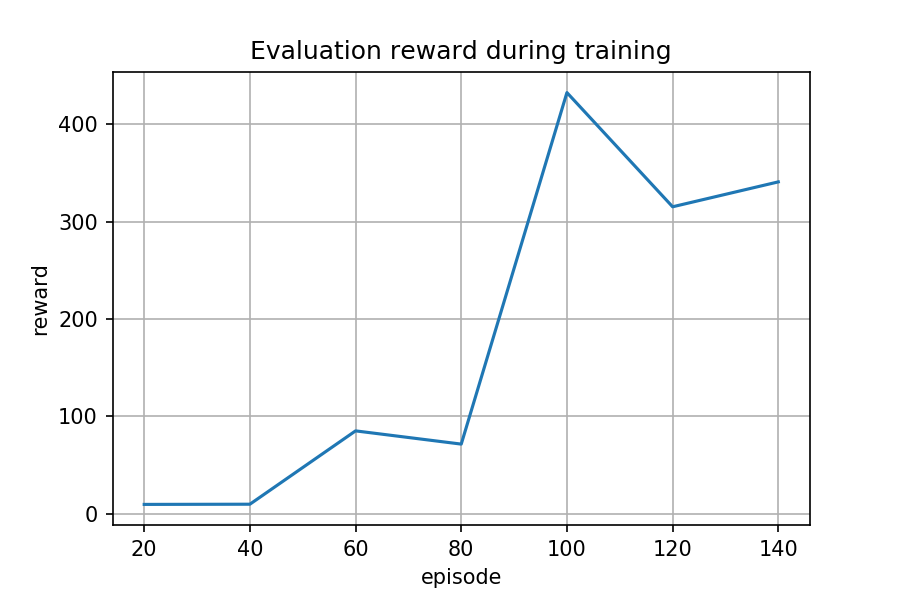
\includegraphics[width=11.70cm, height=7.9cm]{plots/cartpole_evaluation_reward.png}
	\caption{
		\label{fig:cartpole_evaluation_reward}
		Evaluated CartPole agent with deterministic actions every 20th episodes (mean episode reward over 5 episodes).
	}
\end{figure}

\subsection{CarRacing}\label{carracing}

For the CarRacing task we used a convolutional neural network. It consists of three convolutional layers with 32 8x8, 64 4x4 and 64 3x3 filters and strides of 4, 2 and 1. After that a fully connected layer with 256 hidden units is added. Like in \autoref{cartpole} the network is optimized with mean squared error and Adam optimizer. The size of the batches sampled from the replay buffer was 128 and we used a learning rate of 0.0003. \\

For training improvement we skipped four frames and repeated the agents action during this time. For the exploration we set different probabilities for the five actions so the agent prefers the actions accelerate and going straight over the other actions.\\

\autoref{fig:carracing_episode_reward} shows the achieved reward during the training episodes. During training every 20th episode the agent was evaluated with deterministic actions over 5 episodes. The average reward of these 5 episodes is shown in \autoref{fig:carracing_evaluation_reward}. The final performance was evaluated over 15 test episodes. Here the average reward was 559 with a standard deviation of 217. During testing we saw that the agent was able to follow the track but had problems with the sharp curves. For these curves the agent was to fast and didn't slow down.

\begin{figure}[H]
	\centering 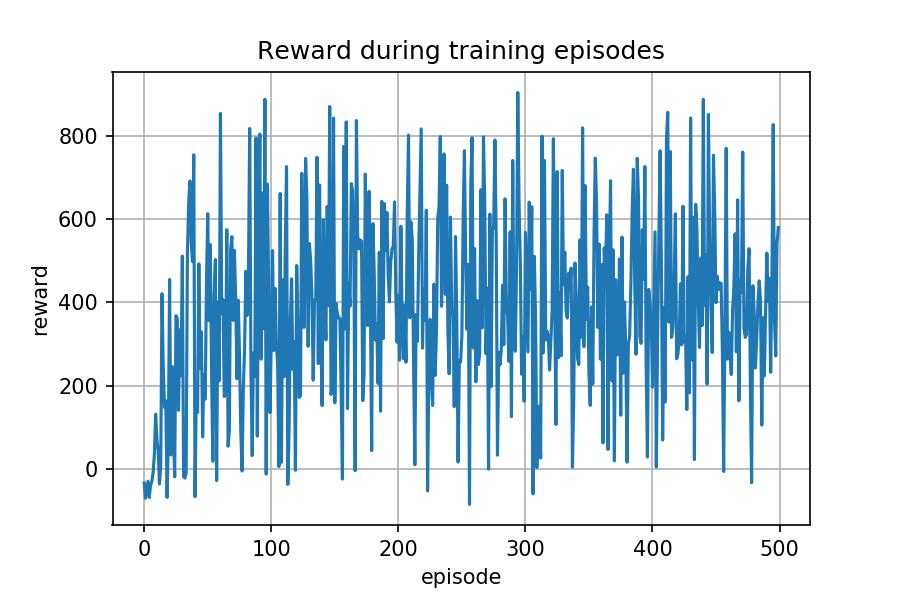
\includegraphics[width=11.70cm, height=7.9cm]{plots/carracing_episode_reward.png}
	\caption{
		\label{fig:carracing_episode_reward}
		Achieved reward during training episodes of CarRacing.
	}
\end{figure}

\begin{figure}[H]
	\centering 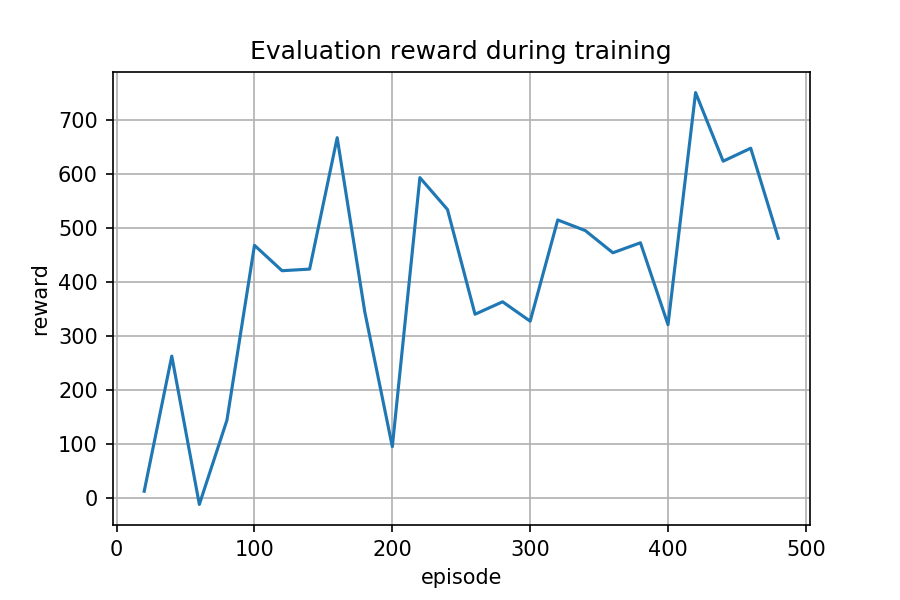
\includegraphics[width=11.70cm, height=7.9cm]{plots/carracing_evaluation_reward.png}
	\caption{
		\label{fig:carracing_evaluation_reward}
		Evaluated CarRacing agent with deterministic actions every 20th episodes (mean episode reward over 5 episodes).
	}
\end{figure}

\section{Exploration}

As a final task we wanted to test how the agent performs if we use $\epsilon$-annealing so that the agent explores more at the beginning of training. We used the same architecture and parameters as described in the carracing section and trained another carracing agent. To let the agent explore more of its environment we started with an $\epsilon$ of 0.5 and gradually decreased it to 0.05 after 100 episodes (every 20th episode a decrease of 0.1 and 0.05 from episode 100 to the end). We also changed the number of maximum time steps per episode during an earlier stage of the training. For episode 0 to 59 the agent used a maximum of 250 timesteps, from episode 60 to 99 maximally 500 timesteps and the usual 1000 timesteps after that.  We chose this range of episodes since we saw in the training before that the agent did not learn very much in the first 50 episodes but had learned how to drive on the road for some time after 100 episodes even without much exploration. 

Moreover we tested the agent's deterministic policy every 10th episode. You can see the rewards during training, for both training episodes as well as the deterministic episodes in between, in Figure \ref{fig:carracing_eps_agent}. We tested the agent's final performance in 15 test episodes where the agent achieved a mean reward of 632 with a standard deviation of 228. 

\begin{figure}[H]
	\centering 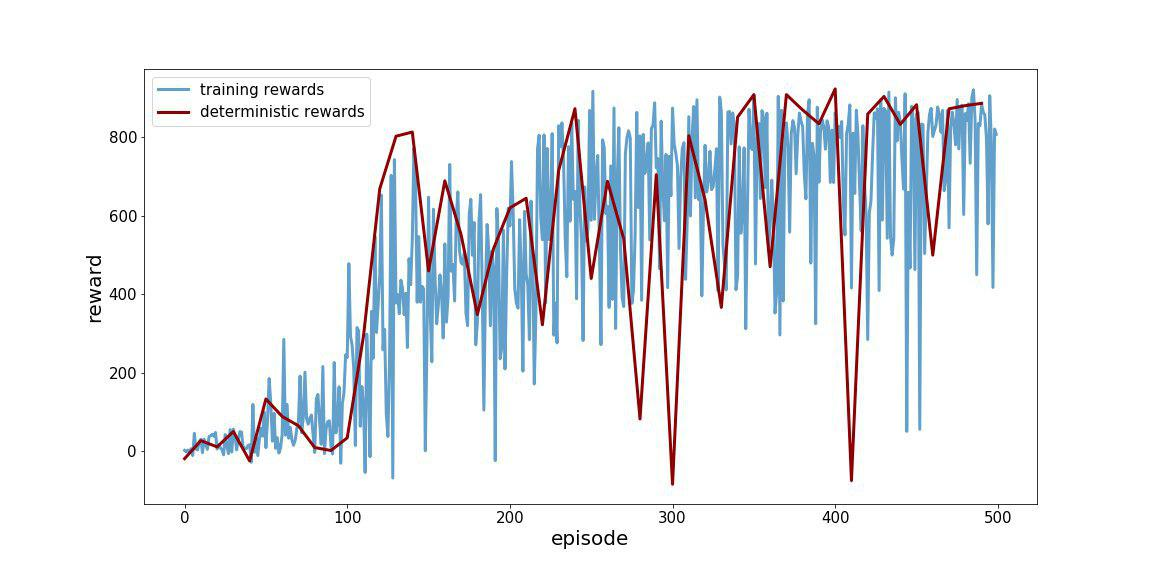
\includegraphics[width=15.5cm, height=7.9cm]{plots/eps_annealing_agent_rewards.jpg}
	\caption{
		\label{fig:carracing_eps_agent}
		Carracing rewards during training episodes and deterministic episodes for agent with epsilon annealing.
	}
\end{figure}


\section{Conclusion}
If you compare the results from the carracing agent with and without epsilon annealing there does not seem to be a big difference. The agent with epsilon annealing has a slightly higher mean reward (632 compared to 559), but together with the very high variances of both agents it could very well be that the agent with epsilon annealing is only better due to chance or maybe is not even better but had more luck with the testing tracks. This suspicion is further confirmed when looking at the agents' behavior during the testing episodes. They both have no problems staying on the road for most of the time but when a sharp curve appears they are too fast to stay on the road and sometimes struggle to get back on the road afterwards. 

However, from the training curves (Figures \ref{fig:carracing_eps_agent}, \ref{fig:carracing_episode_reward} and \ref{fig:carracing_evaluation_reward}) we could assume that the agent with epsilon annealing is at least more stable during training since it does not have many training episodes with a reward below 400 after the 200th episode. On the other hand its deterministic episode reward is below 100 a few times which might refute this assumption. For more insight into this topic further tests would be helpful but this clearly goes beyond the scope of this exercise. 



\end{document}
